\documentclass[twoside,twocolumn,10pt]{extarticle}

\usepackage{amssymb}
\usepackage{multirow}
\usepackage{textcase}
\usepackage{amsthm}
\usepackage{amssymb}
%\newtheorem{thm}{Theorem}
\theoremstyle{definition}
%\newtheorem{defn}[thm]{Definition} % definition numbers are dependent on theorem numbers
%\newtheorem{exmp}[thm]{Example}

\usepackage{blindtext} % Package to generate dummy text throughout this template 

\usepackage[sc]{mathpazo} % Use the Palatino font
\usepackage[T1]{fontenc} % Use 8-bit encoding that has 256 glyphs
\linespread{1.05} % Line spacing - Palatino needs more space between lines
\usepackage{microtype} % Slightly tweak font spacing for aesthetics

\usepackage[italian]{babel} % Language hyphenation and typographical rules
\usepackage[utf8]{inputenc}

\usepackage[hmarginratio=1:1,top=32mm,columnsep=20pt]{geometry} % Document margins
\usepackage[hang,small,labelfont=bf,up,textfont=it,up]{caption} % Custom captions under/above floats in tables or figures
\usepackage{booktabs} % Horizontal rules in tables
\usepackage{subcaption}

\usepackage{graphicx}
\usepackage{float}
\usepackage{listings}
\usepackage{color}
\usepackage{textcomp}

\definecolor{codegreen}{rgb}{0,0.6,0}
\definecolor{codegray}{rgb}{0.5,0.5,0.5}
\definecolor{codepurple}{rgb}{0.58,0,0.82}
\definecolor{backcolour}{rgb}{0.95,0.95,0.92}

\lstdefinestyle{mystyle}{
	backgroundcolor=\color{backcolour},   
	commentstyle=\color{codegreen},
	keywordstyle=\color{magenta},
	numberstyle=\tiny\color{codegray},
	stringstyle=\color{codepurple},
	basicstyle=\footnotesize,
	breakatwhitespace=false,         
	breaklines=true,                 
	captionpos=b,                    
	keepspaces=true,                 
	numbers=left,                    
	numbersep=5pt,                  
	showspaces=false,                
	showstringspaces=false,
	showtabs=false,                  
	tabsize=2
}
\lstset{style=mystyle}

\usepackage{lettrine} % The lettrine is the first enlarged letter at the beginning of the text

\usepackage{enumitem} % Customized lists
\setlist[itemize]{noitemsep} % Make itemize lists more compact

\usepackage{abstract} % Allows abstract customization
\renewcommand{\abstractnamefont}{\normalfont\bfseries} % Set the "Abstract" text to bold
\renewcommand{\abstracttextfont}{\normalfont\small\itshape} % Set the abstract itself to small italic text

\usepackage{titlesec} % Allows customization of titles
\renewcommand\thesection{\Roman{section}} % Roman numerals for the sections
\renewcommand\thesubsection{\roman{subsection}} % roman numerals for subsections
\titleformat{\section}[block]{\large\scshape\centering}{\thesection.}{1em}{} % Change the look of the section titles
\titleformat{\subsection}[block]{\large}{\thesubsection.}{1em}{} % Change the look of the section titles

\usepackage{fancyhdr} % Headers and footers
\pagestyle{fancy} % All pages have headers and footers
\fancyhead{} % Blank out the default header
\fancyfoot{} % Blank out the default footer
\fancyhead[C]{Apprendimento per Rinforzo $\bullet$ Maggio 2017 $\bullet$ \textit{Machine Leargning}} % Custom header text
\fancyfoot[RO,LE]{\thepage} % Custom footer text

\usepackage{titling} % Customizing the title section

\usepackage{hyperref} % For hyperlinks in the PDF

% Title Section
\setlength{\droptitle}{-4\baselineskip} % Move the title up

\pretitle{\begin{center}\Huge\bfseries} % Article title formatting
\posttitle{\end{center}} % Article title closing formatting
\title{Apprendimento per Rinforzo:\\Agente Deep Q\texttwelveudash Network e\\ Casi di Inefficacia} % Article title
\author{%
\textsc{Maxim Gaina e Bartolomeo Lombardi} \\[1ex] % Your name
\normalsize Università di Bologna\thanks{Progetto per il corso di Complementi di Linguaggi di Programmazione, A.A. 2016/2017, prof. Andrea Asperti.} \\ % Your institution
\normalsize \href{mailto:maxim.gaina@studio.unibo.it}{\{maxim.gaina, bartolomeo.lombardi\}@studio.unibo.it}
%\and % Uncomment if 2 authors are required, duplicate these 4 lines if more
%\textsc{Jane Smith}\thanks{Corresponding author} \\[1ex] % Second author's name
%\normalsize University of Utah \\ % Second author's institution
%\normalsize \href{mailto:jane@smith.com}{jane@smith.com} % Second author's email address
}
\date{\today} % Leave empty to omit a date
\renewcommand{\maketitlehookd}{%
\begin{abstract}
\noindent Data la rete neurale Deep Q\texttwelveudash Network ideata e implementata da DeepMind, l'obiettivo di questo lavoro di progetto consiste nel comprendere per quale motivo tale agente, in breve DQN, ha ottenuto risultati sotto la soglia delle prestazioni umane su un sottoinsieme del parco giochi Atari 2600. Verrà quindi studiato l'Apprendimento per Rinforzo, l'algoritmo Q\texttwelveudash Learning e la sua evoluzione DQN assieme all'architettura delle reti neurali sottostanti; in maniera aggiuntiva, pur non disponendo delle stesse risorse di calcolo, si cercheranno di fare delle prove pratiche in grado di mimare i risultati ottenuti precedentemente, analizzandoli. Infine verrà dato uno sguardo a quali sono state le innovazioni in questo ambito.
\end{abstract}
}

\begin{document}

\maketitle

\tableofcontents

\section*{Introduzione}
	\lettrine[nindent = 0.4em,lines=3]{N}\space\MakeTextLowercase{e}ll'ambito del \textit{Machine Learning} si possono individuare diversi stili nella risoluzione dei problemi. L'apprendimento \textit{supervisionato} prevede che a un modello vengano forniti esempi di input e relativi output, affinché esso individui delle regole in grado di mappare input futuri nella maniera più corretta possibile. Esistono diverse metriche in grado di individuare le prestazioni di un modello. L'apprendimento \textit{non supervisionato} invece, ammette che al modello vengano forniti dati non etichettati. Il suo compito sarà poi quello di individuare autonomamente dei pattern o delle features. Il tipo di apprendimento che viene preso in considerazione in questo progetto è l'apprendimento \textit{per rinforzo} (\textit{Reinforcement Learning, RL}). Si può dire che gli algoritmi RL interagiscono con ambienti dinamici in cui ci sono degli obiettivi da raggiungere, per poi ricevere un feedback sotto forma di \textit{premio} o \textit{punizione}. In altre parole, ci sono degli input e degli output etichettati come nell'apprendimento supervisionato, ma le etichette dei dati in output cambiano per adattarsi meglio all'ambiente.
	
	Una tecnica per affrontare i problemi RL è l'algoritmo \texttt{Q\texttwelveudash Learning} che, preso singolarmente, in alcuni casi presenta imperfezioni e persino comportamenti divergenti. È stato formalizzato e implementato dalla \textit{start-up} DeepMind un agente in grado di imparare a giocare all'intero parco titoli di Atari 2600, tramite reti neurali deep che approssimano l'algoritmo \textit{Q\texttwelveudash Learning}. Quest'ultimo però, per risolvere i problema legati alla sua stabilità, è stato modificato inserendo il concetto di \textbf{Experience Replay} e altre modifiche che verranno citate più tardi. È necessario capire la motivazione fondamentale dietro a questi sforzi, cioè quella di creare un singolo algoritmo in grado di affrontare un'ampia varietà di problemi, che a sua volta è da sempre un obiettivo dell'Intelligenza Artificiale Generale. Un unico modello che affronta un intero parco giochi è un ottimo allenamento: per la maggior parte dei giochi Atari 2600 sono stati ottenuti risultati brillanti. Esiste tuttavia un insieme di giochi in cui l'agente \textit{Deep Q\texttwelveudash Network} (DQN) non supera le prestazioni umane o non migliora le metriche ottenuti da metodi precedentemente usati. In questo progetto si prenderà uno dei giochi in cui l'agente DQN non si dimostra particolarmente bravo e si cercherà di capire perché.
	
	La relazione è strutturata in questo modo:
	\begin{itemize}
		\item nella prima sezione verrà descritto l'algoritmo Q\texttwelveudash Learning e le aggiunte fatte dall'agente Deep Q\texttwelveudash Network;
		\item la seconda sezione descriverà l'architettura delle reti neurali sottostante all'agente DQN;
		\item DISCORSO SINCRONIA ASINCRONIA
	\end{itemize}
	
\section{Agente DQN}\label{sec:dqn-agent}
	In questa sezione verrà descritto in breve l'algoritmo \textit{Q\texttwelveudash Learning} (QL), e in che modo l'agente DQN ne riprende il concetto e come quest'ultimo sia stato definito.

	\subsection{Algoritmo Q\texttwelveudash Learning}
		L'algoritmo si basa su una funzione di questo tipo:
		\begin{center}
			$Q: S\times A \longrightarrow \mathbb{R}$,
		\end{center}
		dove $S$ è l'insieme degli stati che può assumere l'ambiente dinamico e $A$ sono le possibili azioni da eseguire. Dopo aver eseguito un'azione $a \in A$ l'agente si muove verso il prossimo stato ricevendo una ricompensa. Tuttavia, l'algoritmo deve imparare quale azione $a$ sia \textit{ottimale} per ogni stato, perché il suo obiettivo ultimo è quello di massimizzare la quantità totale di ricompense ricevute. Per azione ottimale si intende quella che a lungo termine ha la ricompensa più alta. Il QL è un algoritmo iterativo, sono quindi necessarie delle condizioni iniziali. L'apprendimento parte ritornando un valore predefinito, e ogni volta che agisce osserva un nuovo stato insieme alla ricompensa che possono dipendere dallo stato precedente e dall'azione selezionata, aggiornando il valore di $Q$.
		\begin{figure*}[ht]
			\begin{equation}\label{eq:q-learning}
			Q(s_t, a_t) := Q(s_t, a_t) + \alpha_t \cdot (r_{t + 1} + \gamma \cdot \max_a Q(s_{t + 1}, a) - Q(s_t, a_t))
			\end{equation}
			\begin{equation}\label{eq:reward}
				R_t = \sum_{t' = t}^{T} \gamma^{t' - t} r_{t'}
				% dove $T$ è il tempo di termine del gioco.
			\end{equation}
			\begin{equation}\label{eq:dqn-learning}
			Q^*(s, a) = \max_\pi \mathbb{E} [R_t | s_t = s, a_t = a, \pi]
			\end{equation}
		\end{figure*}
		L'equazione \ref{eq:q-learning} descrive l'algoritmo QL.
		
		\paragraph*{Learning rate $\alpha_t$}\label{par:lr} O anche \textit{tasso di apprendimento}, viene usato per regolare quanto un nuovo aggiornamento incide su quello che è già stato appreso, e si ha che $0 \leq \alpha_t \leq 1$. Infatti il valore $0$ è un estremo che indica che l'algoritmo non memorizzerà nulla, mentre il valore $1$ specifica che bisogna memorizzare solo le informazioni più recenti.
		
		\paragraph*{Discount factor $\gamma$}\label{par:gamma} Oppure \textit{fattore di sconto}, che aiuta a determinare l'importanza delle ricompense ricevute. Analogamente a prima si ha che $0 \leq \gamma \leq 1$, dove lo zero imposta l'attenzione dell'algoritmo sulle ricompense immediate, mentre il valore $1$ induce a scelte in funzione di ricompense migliori a lungo termine.
		
		\paragraph*{Ricompensa $r_{t + 1}$}\label{par:reward} Infine, $r_{t + 1}$ indica la ricompensa stessa dopo aver eseguito $a$ dentro a $s_t$. La ricompensa è una sommatoria pesata dei valori attesi di ricompense ottenibili dagli \textbf{step} futuri a partire dallo stato corrente, e per i futuri $\Delta t$ step i pesi sono calcolati da $\gamma^{\Delta t}$.
		
		È detto \textbf{episodio} dell'algoritmo la sequenza di stati che termina con uno stato finale. In un videogioco l'episodio si può vedere come il tentativo di raggiungere un obbiettivo, o completare un livello, che può finire con fallimento e successo. Solitamente è necessario un ampio numero di episodi prima che l'agente sia in grado di fare qualcosa di accettabile. Le implementazioni dell'algoritmo QL sono varie, ma la forma più semplice si basa su una tabella in cui le righe possono essere gli stati e le colonne le azioni. Ogni cella $Q_{i, j}$ contiene il valore di quanto sia ottimale l'azione $a_j$ nello stato $s_i$, e tale valore viene aggiornato opportunamente. Tuttavia, è un metodo non applicabile ad ambienti complessi in cui il numero degli stati è enorme. Un'altro modo è quello di approssimare la funzione tramite Reti Neurali Deep, ed è questa la strada che imbocca l'agente DQN che verrà visto fra poco.
		
		\paragraph{Limiti di Q\texttwelveudash Learning} Anche se l'algoritmo QL appena accennato è stato prima introdotto e ne è stata poi dimostrata la convergenza, esso è conosciuto per il suo comportamento potenzialmente divergente se la funzione Q viene rappresentata da un approssimatore non lineare come le reti neurali. Come riportato in \cite{bib:dqn}, uno dei problemi è che piccoli cambiamenti a Q possono cambiare significativamente la distribuzione dei dati, in più si aggiunge la correlazione fra sequenze di osservazione; insieme alla correlazione fra il vecchio valore $Q(s_t, a_t)$ e il nuovo valore appreso (nella letteratura spesso denominato come Q\texttwelveudash target o \textbf{target value}) $r_{t + 1} + \gamma \cdot \max_a Q(s_{t + 1}, a)$ facente parte dell'equazione \ref{eq:q-learning}. La correlazione tra valori consecutivi non porta a buoni risultati.
		
	\subsection{Deep Q\texttwelveudash Network}
		L'agente \textit{Deep Q\texttwelveudash Network} (DQN) ha come base l'algoritmo QL precedentemente descritto. QL infatti è fondato sulla versione iterativa dell'equazione di Bellman, che a sua volta si basa sulla seguente intuizione: se il valore ottimale di una sequenza di coppie \textit{(azione, osservazione)} fosse conosciuta per ogni possibile azione prossima, allora la strategia ottimale è quella di scegliere l'azione che massimizza il valore atteso del valore appreso $r_{t + 1} + \gamma \cdot \max_a Q(s_{t + 1}, a)$. Le aggiunte fondamentali del DQN però sono le seguenti:
		\begin{enumerate}
			\item \textit{Convolutional Neural Network} (CNN) per approssimare il massimo guadagno possibile seguendo una determinata politica $\pi$ (distribuzione delle probabilità su azioni da eseguire) \ref{eq:dqn-learning}, e dove viene fatto riferimento alla ricompensa in un determinato istante, $R_t$, definito dalla \ref{eq:reward} dove $T$ è il tempo di fine partita;
			\item \textit{Experience Replay}, un meccanismo che permette di allenare la CNN usando ricordi tratti da esperienze passate;
			\item un nuovo metodo di aggiornamento dei valori di Q, usando una seconda rete neurale deep.
		\end{enumerate}
		Gli autori hanno anche dimostrato che togliendo anche uno solo di questi tre elementi i risultati peggiorano drasticamente. Seguiranno le spiegazioni più dettagliate dei cambiamento apportati.

		La funzione Q viene parametrizzata così diventando
		\begin{center}
			$Q(s, a; \Theta_i)$,
		\end{center}
		dove $\Theta_i$ sono i pesi della rete convoluzionale durante l'iterazione $i$-esima, e vengono aggiustati ad ogni iterazione per minimizzare l'errore quadratico nell'equazione di Bellman, dove le etichette vengono approssimate da
		\begin{center}
			$y = r + \gamma \max_{a'} Q(s', a'; \Theta_i^-)$,
		\end{center}
		con $\Theta_i^-$ che sono i parametri dello step precedente. La rete deep in questione viene anche chiamata Q\texttwelveudash Network. Come è già stato accennato, le etichette dipendono dai pesi della rete (al contrario di quanto si usa nell'apprendimento supervisionato), e la funzione costo (\textit{loss function}) cambia ad ogni iterazione $i$. Senza riscrivere tutti i passaggi matematici della lettera originale, ci limitiamo a riportare la funzione costo derivata rispetto ai pesi (equazione \ref{eq:gradient-loss}).
		\begin{figure*}
			\begin{equation}\label{eq:gradient-loss}
				\nabla_{\Theta_i} L(\Theta_i) = \mathbb{E}_{s, a, r, s'} [(r + \gamma \max_{a'} Q(s', a'; \Theta_i^-)) \nabla_{\Theta_i} Q(s, a; \Theta_i)]
			\end{equation}
		\end{figure*}
		Per bilanciare fra loro i fattori \textit{exploration} ed \textit{exploitation} nello spazio comportamentale in un determinato stato, l'algoritmo seleziona $a$ in maniera casuale con una probabilità $\epsilon$, oppure segue la politica $\pi$ con una probabilità $1 - \epsilon$, dove $\epsilon$ è determinato sperimentalmente.

		\paragraph*{Experience Replay (ER)}\label{par:er} Ad ogni passo di tempo $t$ viene archiviata l'esperienza dell'agente costituita dalla tupla $e_t = (s_t, a_t, r_t, s_{t + 1})$, che esprime rispettivamente lo stato in cui ha scelto una determinata azione, la ricompensa ricevuta e lo stato di arrivo. L'insieme delle esperienze è $D$, ed esso accumula esperienze di molteplici episodi fino a un determinato numero $N$ (l'esperimento originario ne accumula un milione). Ogni volta che un \textit{minibatch} fornisce una nuova quantità di esperienze, ne vengono raccolte altrettante nell'insieme $D$ e vengono aggiornate con quelle nuove. In breve, seguono alcuni vantaggi nell'utilizzo dell'ER:
		\begin{itemize}
			\item ogni esperienza può essere usata in molteplici aggiornamenti dei pesi della Q\texttwelveudash Network;
			\item rendere casuale il campionamento di esperienze da aggiornare rompe la correlazione fra eventi consecutivi.
		\end{itemize}
	
		\paragraph*{Q\texttwelveudash Network Separata} L'altra modifica è quella di aggiungere un'ulteriore rete deep per generare i label $y_i$. Ogni $C$ aggiornamenti la funzione $Q$ viene clonata come $\hat{Q}$, dove $\hat{Q}$ verrà usata per generare etichette $y_i$ per $Q$ per i prossimi $C$ passi. Anche questo è un accorgimento per evitare ciò che accade nel Q\texttwelveudash Learning classico dove, un incremento di $Q(s_t, a_t)$ influisce su $Q(s_t, a)$ per qualsiasi valore di $a$ e quindi per tutte le etichette $y_i$. Così facendo viene quindi viene evitata la divergenza dalla politica comportamentale $\pi$.
		
	\subsection{Implementazione in LUA}
		Il linguaggio usato da \textit{DeepMind} per l'implementazione dell'algoritmo DQN è \texttt{LUA}. Si tratta di un linguaggio di programmazione che punta su efficienza e \textit{leggerezza}, e supporta diversi paradigmi come la programmazione procedurale, orientata agli oggetti, funzionale e programmazione descrittiva dei dati. \texttt{LUA} è noto per essere usato in ambiti ludici (\textit{World of Warcraft} e molti giochi per android sono scritti in \texttt{LUA}) e, a quanto pare anche \textit{DeepMind}, avendo a che fare con i videogiochi, non si è allontanata troppo dal trend.
		
		\paragraph*{Dipendenze} Per metterci le mani sopra, è stata usata una fork del codice originario che permette di vedere anche graficamente sia l'apprendimento che l'esecuzione dei test\footnote{DeepMind Atari Q\texttwelveudash Learner, \emph{\href{https://github.com/kuz/DeepMind-Atari-Deep-Q-Learner}{GitHub Repository.}}}. In breve, sono state usate le seguenti principali dipendenze:
		\begin{itemize}
			\item \textit{Xitari}, fork di \textit{The Arcade Learning Envoirnment}\footnote{ALE, \emph{\href{http://www.arcadelearningenvironment.org/}{Arcade Platform for General Artificial Intelligence development.}}} che permette a chiunque di sviluppare agenti di intelligenza artificiale in grado di interfacciarsi con l'emulatore Atari 2600 \textit{Stella}\footnote{Stella, \emph{\href{https://github.com/stella-emu/stella}{Atari 2600 Emulator.}}};
			\item \texttt{AleWrap}, interfaccia \texttt{LUA} per \texttt{Xitari};
			\item \texttt{LuaJIT}, compilatore \textit{Just in Time} per \texttt{LUA};
			\item \texttt{Torch 7.0}, framework per computazioni di carattere scientifico e ampio supporto ad algoritmi di apprendimento automatico;
			\item \texttt{nn}, libreria potente per fornire un metodo facile e modulare per costruire e allenare reti neurali (molto simile a \texttt{Keras} con i suoi modelli sequenziali).
		\end{itemize}
	
		È possibile allenare il proprio agente usando le proprie \texttt{CPU} o \texttt{GPU} (o una in particolare) tramite i relativi script. Ogni script contiene i seguenti iperparametri (parametri che servono prima del lancio): passi da eseguire, ogni quanti passi eseguire la validazione, valore iniziale di $\gamma$ ed $\epsilon$, learning rate ed altri parzialmente riportati nella Figura \ref{code:run}. L'implementazione in \texttt{LUA} è abbastanza corposa quindi verranno ora riportate le parti ritenuti fondamentali.
		\begin{figure*}[ht!]
			\centering
			\caption{Parte dello script di lancio \texttt{run\_cpu}}
			\lstinputlisting{code/run}
			\label{code:run}
		\end{figure*}
	
		\subsubsection{train\_agent}
			Si tratta del file con codice \texttt{LUA} che:
			\begin{itemize}
				\item contiene la ricezione e l'elaborazione degli iperparametri visti prima;
				\item viene creato l'ambiente del gioco selezionato (possibili ricompense e possibili azioni) e viene istanziato l'agente con tutte le sue opzioni;
				\item a tempo di esecuzione vengono mantenute tutte le informazioni riguardarni il tempo stesso di esecuzione, numero di ricompense, numero di episodi e di step già fatti, e così via;
			\end{itemize}
			Ma l'importanza di \texttt{train\_agent} nella gerarchia dei file sorgente è data dalla presenza del ciclo che itera i passi di apprendimento fino al massimo dichiarato (che di default ricordiamo essere $50mln$). Dato che il ciclo contiene parecchio codice, viene riportata la sua versione riassuntiva nella figura \ref{code:tagent}.
			\begin{figure*}[ht!]
				\centering
				\caption{Ciclo \texttt{while} fondamentale riportato in maniera riassuntiva nel file \texttt{training\_agent}}
				\lstinputlisting[language={[5.0]Lua}]{code/tagent.lua}
				\label{code:tagent}
			\end{figure*}
		
		\subsubsection{NeuralQLearner}
			Alla riga $7$ in Figura \ref{code:tagent} che riporta il ciclo while nel file \texttt{train\_agent}, è presente il metodo
			\begin{verbatim}
				perceive(reward, screen, terminal).
			\end{verbatim}
			Esso appartiene a \texttt{NeuralQLearner.lua}. Si tratta dell'implementazione stessa dell'algoritmo DQN, di conseguenza ecco quanto accade qui alla sua istanziazione:
			\begin{itemize}
				\item gli iperparametri vengono usati per inizializzare la rete convoluzionale di cui si parlerà più tardi in \ref{sec:cnn};
				\item vengono inizializzati i parametri che regolano il comportamento \textbf{exploration vs. exploitation} (cioè $\epsilon$ e relativi parametri di raffreddamento durante il processo di apprendimento)
				\item inizializzazione e raffreddamento del \textit{learning rate} (visto in \ref{par:lr});
				\item il così detto \texttt{discount factor}, che in realtà è il valore $\gamma$ visto in \ref{par:gamma};
				\item istanziazione della classe \texttt{TransitionTable}, che in realtà l'implementazione dell'insieme $D$ contenente le esperienze, visto in \ref{par:reward};
				\begin{verbatim}
					self.transitions = 
					         dqn.TransitionTable(args)
				\end{verbatim}
				\item e altri parametri relativi al massimo e minimo della ricompensa, ecc...
			\end{itemize}
			
			Riteniamo importante ora elencare i principali metodi di \texttt{NeuralQLearner}, che modificano iterativamente i parametri e i valor inizializzati elencati appena sopra:
			\begin{enumerate}
				\item 	
				\begin{verbatim}
					preprocess(rawstate)			
				\end{verbatim}
					Prende in input l'immagine grezza perché poi sia pronta per essere elaborata dalla rete (preprocesamento spiegato in \ref{subsubsec:preproc});
				\item 
				\begin{verbatim}
					getQUpdate(args)
				\end{verbatim}
					Per ogni azione viene ritornato l'aggiornamento del valore Q, ricordiamo che la rete neurale approssima il valore ottimale per ogni azione disponibile. Si tratta di un'iterazione espressa dall'equazione \ref{eq:dqn-learning};
				\item
				\begin{verbatim}
					qLearnMinibatch
				\end{verbatim}
					Dopo aver ottenuto il nuovo valore di Q invocando \texttt{getQUpdate(args)}, il metodo aggiorna i pesi della rete neurale tramite il calcolo del gradiente, in base al minibatch di nuove esperienze che poi verranno salvate anche nella \texttt{TransitionTable}. Questo è quanto esprime l'equazione \ref{eq:gradient-loss}.
				\item 
				\begin{verbatim}
					perceive(reward, rawstate, terminal
					         testing, testing_ep)
				\end{verbatim}
					Il metodo \texttt{perceive(args)} esprime la principale iterazione e quindi viene riportato nella Figura 
				\item
				\begin{verbatim}
					eGreedy(state, testing_ep)
				\end{verbatim}
					Dato il valore aggiornato di $\epsilon$, prende un valore casuale che se è minore di $\epsilon$ ritorna la prossima azione come casuale, altrimenti invoca il metodo \texttt{greedy(state)};
				\item
				\begin{verbatim}
					greedy(state)
				\end{verbatim}
					Dato lo stato, valuta tutte le azioni possibili e ritorna l'azione ritenuta ottimane.
			\end{enumerate}

\begin{figure*}[h]
	\centering
	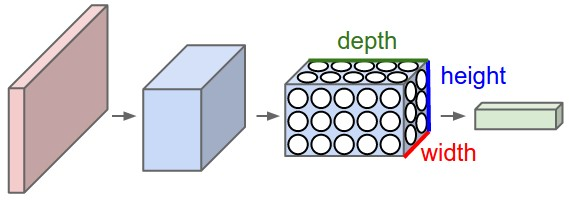
\includegraphics[scale=.5]{images/cnn.jpeg}
	\caption{Neuroni di una CNN}
	\label{fig:cnn}
\end{figure*}

\begin{figure*}[h]
	\centering
	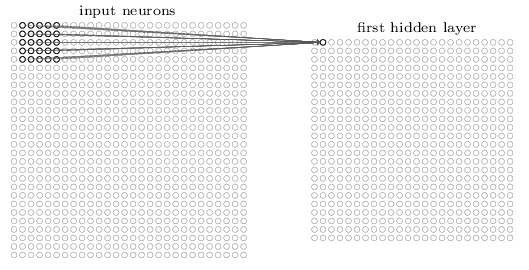
\includegraphics[scale=.5]{images/hlayer.jpeg}
	\caption{Local receptive fields}
	\label{fig:hlayer}
\end{figure*}

\section{Reti Neurali Convoluzionali}\label{sec:cnn}
Le reti neurali convoluzionali (CNN) sono usate con grande successo per problemi di riconoscimento automatico di pattern bidimensionali come la rivelazione di oggetti, facce e loghi nelle immagini. Le normali reti neurali stratificate con un'architettura Fully Connected (FC), dove ogni neurone di ciascun layer è collegato a tutti i neuroni del layer precedente (neuroni bias esclusi), in generale non scalano bene con l'aumentare delle dimensioni delle immagini. Le CNN sono costituite da neuroni collegati tra loro tramite rami pesati e anche per questa tipologia di rete i parametri allenabili sono: \textit{weight} e \textit{bias}. La fase di allenamento di una rete neurale attraverso \textit{forward/backward propagation} e aggiornamento dei \textit{weight}, vale anche in questo contesto. 

Le CNN prendono vantaggio dal fatto che l'input consiste in immagini e quindi vincolano l'architettura in modo più sensibile. A differenza di una normale rete neurale, gli strati di un CNN hanno neuroni disposti in tre dimensioni: larghezza, altezza e profondità. Inoltre, i neuroni di un layer sono connessi solo ad una piccola regione del layer precedente, invece che a tutti i neuroni come in un'architettura FC.
Questa è la principale caratteristica che contraddistingue una CNN da una normale rete neurale stratificata con un'architettura fully connected. In figura \ref{fig:cnn} si può vedere come vengono disposti i neuroni all'interno di una CNN, infatti ciascun layer trasforma un volume 3D di input in un volume 3D di output; quest'ultimo costituisce l'insieme delle attivazioni dei neuroni di tale layer, tramite una determinata funzione di attivazione differenziabile.

Questa tipologia di rete usa principalmente tre idee di base: \textit{local receptive fields}, \textit{shared weights and biases} e \textit{pooling}. 

Consideriamo che i pixel dello strato di input siano connessi con quelli dello strato hidden, ma non tutti, bensì solo alcuni di questi. Ogni neurone del primo strato nascosto è connesso ad una regione (ad esempio 5x5) dello strato di input, questa regione dell'immagine dello strato di input è chiamata \textbf{local receptive field} (figura \ref{fig:hlayer}). Ogni connessione apprende un peso e il neurone a cui è associata la connessione apprende un bias totale. In sostanza ogni singolo neurone esegue la convoluzione e la rete è addestrata ad apprendere i pesi e il valore del bias per minimizzare la funzione di costo. Quindi vengono connesse tutte le regioni dello strato di input ai singoli neuroni nel primo strato nascosto, effettuando di volta in volta uno shift. Così facendo se in input avessimo un'immagine 28x28 e le regioni 5x5 otterremo 24x24 neuroni nello strato nascosto.

Dato che i neuroni del primo strato nascosto condividono pesi e bias, questo significa che saranno in grado di riconoscere la stessa feature, solo collocata diversamente nell'immagine di input. Questo rende le CNN molto adattabili all'invarianza di un'immagine ad una traslazione. Per questa ragione, la mappa di connessioni dallo strato di input a quello nascosto è denominata \textit{feature map}, i pesi \textbf{shared weights} e i bias \textbf{shared bias} perché condivisi. Il vantaggio di condividere i pesi e bias sta nella riduzione dei parametri coinvolti in una rete convoluzionale.

Ovviamente per riconoscere un'immagine sono necessarie più di una feature map, quindi, uno strato convoluzionale completo è fatto da più feature maps.
Una CNN può comporsi di più strati di convoluzione collegati in cascata. L’output di ogni strato di convoluzione è un insieme di matrici di convoluzione (ciascuna generata da una mappa di attivazione). L’insieme di queste matrici definisce un nuovo volume di input utilizzato dalle mappe di attivazione dello strato successivo. Più strati convoluzionali possiede una rete e più feature dettagliate essa riesce ad elaborare.

Le CNN usano anche degli strati di \textbf{pooling} posizionati subito dopo agli strati convoluzionali, questi hanno la funzione di semplificare l'informazione di output dello strato precedente. Uno strato di pooling suddivide le matrici convoluzionali in regioni e seleziona un unico valore rappresentativo (valore massimo \textit{max-pooling} o valore medio \textit{average pooling}) al fine di ridurre i calcoli degli strati successivi e aumentare la robustezza delle feature rispetto alla posizione spaziale. In sostanza il pooling sottocampiona spazialmente ogni mappa di feature di input, ovviamente il pooling viene applicato ad ogni feature maps separatamente.

L'ultimo strato di una CNN è esattamente uguale ad uno qualsiasi dei layer di una classica rete neurale artificiale con architettura FC: collega quindi tutti i neuroni dallo strato di max-pooling a tutti i neuroni di uscita, utili a riconoscere l'output corrispondente.
Questo tipo di layer, a differenza di quanto visto finora nelle reti neurali convoluzionali, non utilizza la proprietà di connettività locale: un FC layer è connesso all'intero volume di input e quindi, come si può immaginare, si avranno moltissime connessioni. L’unico parametro impostabile di questo tipo di layer è il numero di neuroni K che lo costituiscono. Ciò che fa sostanzialmente un FC layer è quello di collegare i suoi K neuroni con tutto il volume di input e di calcolare l’attivazione di ciascuno dei suoi K neuroni.
Il suo output sarà infatti un singolo vettore 1 x 1 x K, contenente le attivazioni calcolate. Il fatto che dopo l’utilizzo di un singolo FC layer si passi da un volume di input, organizzato in 3 dimensioni, ad un singolo vettore di output, in una singola dimensione, fa intuire che dopo l’applicazione di un FC layer non si può più utilizzare alcun layer convoluzionale. La funzione principale dei FC layer nell'ambito delle reti neurali convoluzionali è quello di effettuare una sorta di raggruppamento delle informazioni ottenute fino
a quel momento, esprimendole con un singolo numero (l’attivazione di uno dei suoi neuroni), il quale servirà nei successivi calcoli per la classificazione finale. Solitamente si utilizza più di un layer FC in serie e l’ultimo di questi avrà il parametro K pari al numero di classi presenti nel dataset. I K valori finali saranno infine date in pasto all'output layer, il quale, tramite una specifica funzione probabilistica, effettuerà la classificazione. Combinando insieme queste tre idee avremmo una rete convoluzionale completa, la quale sarà addestrata tramite la discesa del gradiente e l’algoritmo di backpropagation.

Da un certo punto di vista, possiamo dire che una rete CNN, per la classificazione, è un sistema che si compone di due componenti fondamentali:
\begin{itemize}
	\item 
	\textbf{Componente di riconoscimento ed estrazione automatica delle feature}. \\Il riconoscimento avviene mediante applicazione di banchi paralleli di filtri convoluzionali i cui elementi sono appresi automaticamente mediante algoritmo del gradiente discendente (essi corrispondono ai pesi delle connessioni dei neuroni). Intuitivamente questa componente ha come obiettivo quello di apprendere dei filtri che si attivano in presenza di un qualche specifico tipo di feature in una determinata regione spaziale dell’input.
	\item
	\textbf{Componente di classificazione}.
\end{itemize}
L’addestramento di una CNN coinvolge entrambe le componenti in cui i parametri degli elementi costitutivi (p.e. neuroni) sono automaticamente variati al fine di minimizzare una funzione di costo.
La capacità di una CNN può variare in base al numero di strati che essa possiede. Raramente si può trovare un solo strato convoluzionale, a meno che la rete in questione non sia estremamente semplice. Di solito una CNN possiede una serie di strati convoluzionali: i primi di questi, partendo dallo strato di ingresso ed andando verso lo strato di uscita, servono per ottenere feature di basso livello, come ad esempio linee orizzontali o verticali, angoli, contorni vari, ecc; più si scende nella rete, andando verso lo strato di uscita, e più le feature diventano di alto livello, ovvero esse rappresentano figure anche piuttosto complesse come dei volti, degli oggetti specifici, una scena, ecc. In sostanza dunque più strati convoluzionali possiede una rete e più feature dettagliate essa riesce ad 

\begin{figure*}[h]
	\centering
	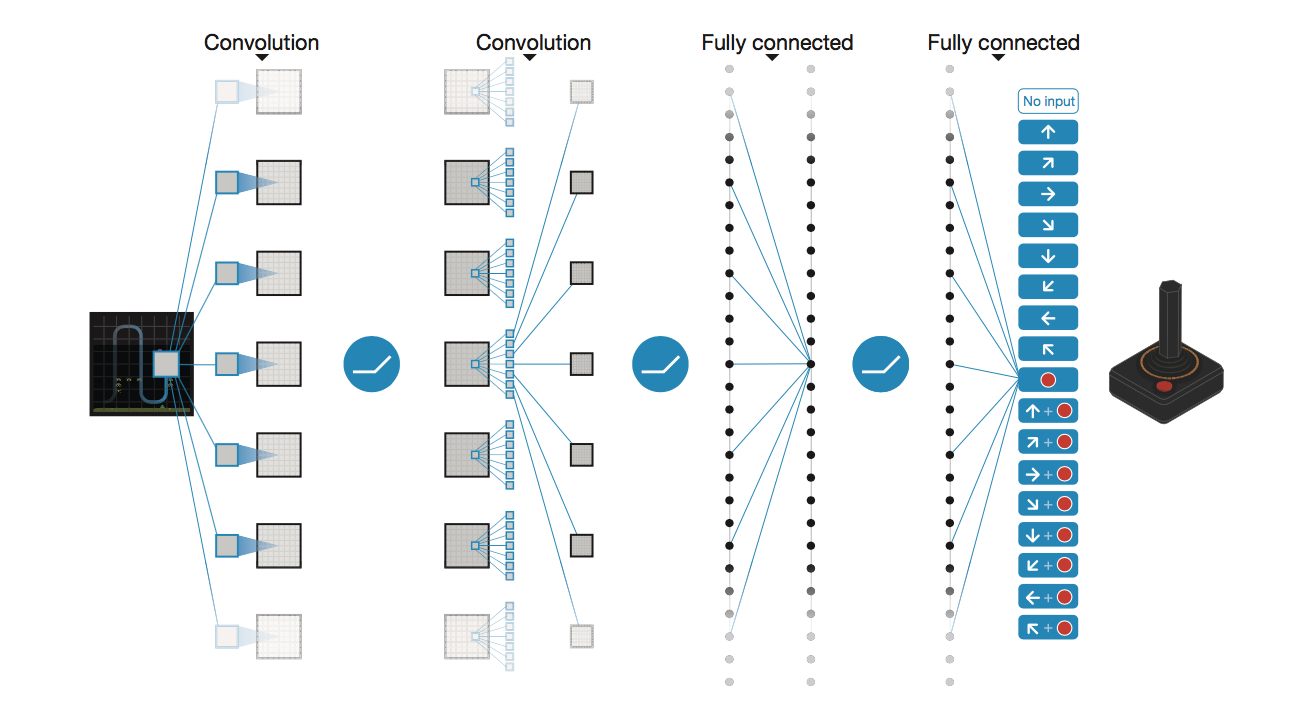
\includegraphics[scale=.2]{images/cnnDQN.jpg}
	\caption{Illustrazione schematica della rete neurale convoluzionale.}
	\label{fig:cnnDQN}
\end{figure*}

\begin{figure*}[ht!]
	\centering
	\lstinputlisting[]{code/fcl.py}
	\caption{Implementazione dei layer convoluzionali}
	\label{fig:layerConv}
\end{figure*}

\begin{figure*}[ht!]
	\centering
	\lstinputlisting[]{code/lfcl.py}
	\caption{Implementazione del layer FC}
	\label{fig:layerFC}
\end{figure*}

\subsection{CNN nel contesto DQN}
\subsubsection{Preprocessing}\label{subsubsec:preproc}
Dopo aver descritto in maniera dettagliata la struttura di una CNN è doveroso delineare il modo in cui l l'agente DQN fa uso di questa rete. Prima di imputare i dati nella CNN, viene eseguito un metodo di \textit{preprocessing} con l'obiettivo di ridurre la dimensione. Dovendo elaborare ogni frame del gioco, dove ogni pixel ha una dimensione di 210 x 160 con una paletta di 128 colori, diventa molto dispendioso in termini di calcolo e requisiti di memoria. Quindi si applica un passo di \textit{preprocessing} di base volto a ridurre la dimensionalità di input e affrontare alcuni artefatti dell'emulatore Atari 2600.
Per codificare un singolo frame, viene tenuto il valore massimo di colore per ogni pixel tra il frame da codificare con quello precedente. Ciò permette di rimuovere il cosiddetto \textit{flickering} presente nei giochi Atari, in cui alcuni oggetti appaiono solo in frame pari mentre altri appaiono solo in frame dispari; un artefatto causato dal numero limitato di "folletti" presenti nei giochi Atari che l'emulatore però visualizza contemporaneamente. Fatto questo, viene poi estratto il canale Y, conosciuto come luminanza, dal frame RGB e viene scalato ad una dimensione di 84 x 84.

\subsubsection{Architettura del modello}
L'architettura schematizzata della rete è mostrata in figura \ref{fig:cnnDQN} ed è strutturata come segue. 
L'input della CNN è un frame che consiste nello snapshot del gioco, con dimensioni 84 x 84 x 4 prodotta dal \textit{preprocessing}. Il primo strato nascosto convoglia 32 filtri di dimensione 8 x 8 con passo 4 dall'immagine di input e viene applicato poi un rectifier (rettificatore) non lineare. Ogni strato nascosto della rete è seguito da uno strato rettificatore che ha come funzione principale quella di incrementare la proprietà di non linearità della funzione di attivazione, accennata in precedenza, senza andare a modificare i receptive field di un layer convoluzionale. Una funzione molto adatta a questo scopo, e per questo è quella utilizzata dai \textit{ReLU} layer, è $f(x) = max(0,x)$.
Il secondo strato nascosto convoglia 64 filtri di dimensione 4 x 4 con passo 2 seguito dallo strato ReLU. Questo è seguito da un terzo strato convoluzionale che convoglia 64 filtri di dimensione 3 x 3 con passo 1 seguito anch'esso da uno strato ReLU. L'ultimo strato nascosto della rete è fully-connected e consiste di 512 unità di rectifier. Lo strato di output è uno strato lineare FC con un singolo ouput per ogni azione valida. Il numero di azioni valide variano fra 4 e 18 nei giochi Atarti considerati dallo studio.

\subsubsection{Implementazione}
Dopo aver descritto l'architettura della CNN utilizzata per questo studio, analizzeremo l'implementazione della struttura. Come accennato in precedenza, il tutto è stato sviluppato in \textit{Lua} con riferimenti a librerie di IA, ma per lo sviluppo della CNN è indispensabile la libreria \textit{Torch}, un framework scientifico di calcolo con ampio supporto per gli algoritmi di machine learning che predilige le GPU. In figura \ref{fig:layerConv} viene mostrata la parte di codice della funzione \textit{create\_network(args)} che implementa i layer convoluzionali con diversi parametri come descritto nella sezione precedente.
L'ultima parte della CNN (figura \ref{fig:layerFC}) vengono implementati gli strati FC, dove vengono collegati tutti i neuroni di uscita, con la funzione principale di effettuare una sorta di raggruppamento delle informazioni ottenute fino a quel momento esprimendole con un singolo numero (l’attivazione di uno dei suoi neuroni), ovvero, l'azione da compiere.

\section{Game Over}\label{}
	L'allenamento dell'agente DQN, spiegato nelle sezioni precedenti e con la stessa struttura della rete, è stato eseguito su $49$ giochi \textit{retro} della console \textit{Atari 2600}. In \cite{bib:dqn} si possono vedere i risultati di tali esperimenti. Quello che sorprende di più è che sono stati raggiunti ottimi risultati per una serie di giochi che in termine di genere hanno poco in comune: si va dagli sparatutto come \textit{River Raid}, passando per \textit{Boxing} e infine i giochi di guida tredimensionali come \textit{Enduro}.
	
	Secondo alcuni criteri gli autori hanno anche stabilito prestazioni sotto o sopra al livello umano. Purtroppo, mentre per circa la metà dei giochi l'agente supera le prestazioni umane in maniera impressionante, ci sono $20$ giochi su $49$ in cui l'agente non riesce a fare meglio. Si vuole provare a individuare il fattore che rende diverse (nei risultati) queste due categorie di giochi, il sospetto è che per come è stato progettato l'algoritmo DQN, esso capti ricompense di alcuni giochi in un modo che non gli permette di imparare comportamenti ottimali.
	
	\subsection{Alcune prove}
		Pur non disponendo neanche lontanamente delle risorse di calcolo a disposizione di \textit{DeepMind}, l'\textbf{intenzione} iniziale era quella di accompagnare lo studio dei risultati non soddisfacenti con alcune prove pratiche, per capire meglio l'ambiente di cui stiamo parlando. Sono state fatte alcune prove su due giochi selezionati da diverse categorie: \textit{Breakout} e \textit{Centipede}. Il primo supera il miglior giocatore umano in maniera che si può definire fuori scala, di ben $1327\%$, mentre il secondo non ha raggiunto risultati soddisfacenti, fermandosi al $62\%$.
		
		Gli step totali eseguiti da \textit{DeepMind} sono $50mln$, che su un PC normale equivale ad aspettare in termini di settimane (o poco più di un mese). In un primo tentativo volevamo vedere cosa succede allenando la rete per soli $700.000$ step, scoprendo che circa $12$ ore ($24$ in totale sia per \textit{Centipede} che \textit{Breakout}) non bastano neanche lontanamente per far emergere qualche comportamento sensato da parte dell'agente. Il punteggio di \textit{Breakout} era di soli $55$ punti (con l'agente sempre fermo alla sinistra dello schermo con qualche tremolio verso destra) mentre la rete allenata per \textit{Centipede} accumulava soli $1811$ punti. In un secondo tentativo di $1,25mln$ di step, ipotizzando che il riempimento della \texttt{TransitionTable} migliorasse in qualche modo la situazione, per solo \textit{Centipede} è stato raggiunto il non molto brillante punteggio di $1911$.
		
		È chiaro che per computazioni del genere in maniera efficiente non basta il computer di casa. Bisogna specificare però che è stata usata la \texttt{CPU} che è un \texttt{i5 4690K}, dato che dopo aver provato due versioni di \texttt{Ubuntu} non risultava essere alcun driver \texttt{CUDA GTX980} compatibile al giorno d'oggi anche con l'implementazione del DQN. Per quanto riguarda il lato pratico quindi, è tutto quello che è stato possibile realizzare.
		
\section{Prestazioni scadenti: cause individuate}
	Prima di tutto era necessario capire l'intero ramo dell'apprendimento per rinforzo, il QL e infine le DQN, fatto ciò è possibile passare allo studio dei risultati presenti in \cite{bib:dqn}. L'attenzione era inizialmente focalizzata sul risultato di \textit{Centipede}, ma per capire il perché delle sue prestazioni non brillanti era anche necessario fare il confronto con altri giochi. Guardando i \textit{gameplay} della maggior parte del parco titoli, e consultando i relativi manuali per capire la natura delle ricompense (\textit{quante} e \textit{quando})\footnote{Atari Age, \emph{\href{https://atariage.com/software_search.php?SystemID=2600}{Atari 2600 Rarity Guide.}}} in relazione alle possibili osservazioni, è risultato chiaro che alcuni giochi in realtà si assomigliano molto per costruzione. Si stava cercando un pattern che distinguesse i giochi in cui l'algoritmo si comportasse bene o male, ma sono stati individuati almeno tre motivi per cui un agente DQN può risultare sotto le prestazioni umane. È necessario ricordare prima di procedere, che la struttura dei giochi non è stata cambiata in alcun modo tranne per il sistema delle ricompense. Qualsiasi ricompensa negativa è stata mappata su $-1$, su $1$ quelle positive e su $0$ quelle nulle. A partire da \cite{bib:dqn} non è chiaro se la fine della partita venga considerato come ricompensa negativa, in seguito ad alcune ricerche nel codice sorgente si nota come in realtà l'agente non venga punito in tal caso:
	\begin{verbatim}
	self.config = {
	...
	gameOverReward = 0,
	...
	}
	\end{verbatim}
	dove la variabile \texttt{gameOverReward} non compare più in alcun assegnamento.

	\subsection{Pianificazione a lungo termine}
		Il punto debole più ovvio di un agente DQN è la pianificazione a lungo termine, in mancanza di ricompense intermedie. Si può facilmente notare nella Figura \ref{fig:montezuma} come, nel gioco \textit{Montezuma's Revenge}, per arrivare a prendere la chiave e quindi ricevere la ricompensa, sia necessario eseguire una lunga catena di azioni diverse e osservazioni senza feedback alcuno. Pensiamo che \textit{Private Eye}, ricalcando le stesse modalità di gioco di \textit{Montezuma's Revenge}, abbia per lo stesso motivo raggiunto un risultato quasi nullo.
		\begin{figure}[ht!]
			\centering
			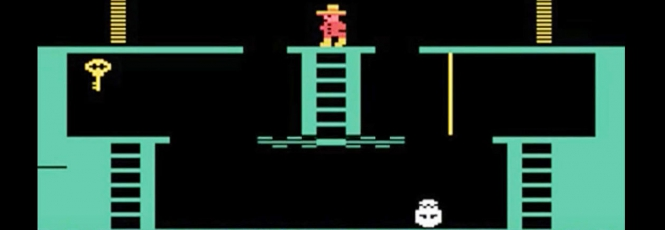
\includegraphics[scale=.31]{images/montezuma.jpg}
			\caption{L'eroe deve arrivare alla chiave eseguendo molteplici azioni ed evitando il teschio.}
			\label{fig:montezuma}
		\end{figure}
		Inoltre, per giocare è necessario muoversi contemporanemante su più livelli, logicamente collegati. Non vediamo alcun meccanismo in grado di gestire scelte del genere.
		
		Almeno per quanto riguarda la singola chiave, si potrebbe ragionare sui valori di $\gamma$; si potrebbe rivedere la velocità di raffreddamento di $\epsilon$ per incentivare ulteriormente l'esplorazione; e si potrebbe ragionare su ricompense intermedie. Ma ricordiamo l'obiettivo è quello di ottenere un algoritmo in grado di apprendere \textit{end-to-end}, di carattere generale, senza il bisogno di modifiche per task specifiche.
		
		Avremmo voluto poter verificare in maniera immediata gli effetti di piccole modifiche sul comportamento dell'agente ma, pur ammettendo di avere capacità di calcolo minimamente paragonabili a quelle a disposizione di \textit{DeepMind}, servirebbero comunque giorni di allenamento per vederne gli esiti.

	\subsection{Scelte di carattere tattico}
		Ci risulta che un'altro punto debole dell'algoritmo proposto da \textit{DeepMind} sia il \textit{fiuto tattico}, che percepiamo come l'abilità di intuire la possibilità di uno scenario sfavorevole e reagire di conseguenza. Non c'è un meccanismo in grado incoraggiare tale comportamento, è vero che l'agente viene punito se va contro il fantasma, ma questi cambiano spesso direzione e (casualmente o no) creano delle zone trappola. Per esempio, si osservi la Figura \ref{fig:subpacman}: una sfavorevole situazione evitabile da prima facendo azioni migliori. Purtroppo, anche in questo caso l'agente DQN otterrebbe tutte le ricompense che gli spettano, senza una previsione iniziale della direzione del fantasma. Un essere umano rimane più bravo a indirizzare \textit{Pac-Man} in una parte del labirinto in cui non ci sono punti da guadagnare, per poi tornare nella parte interessante del labirinto sotto una condizione più favorevole (Figura \ref{fig:subpacman1}).
		
		\begin{figure}[ht!]
			\centering
			
			\begin{subfigure}[b]{.49\textwidth}
				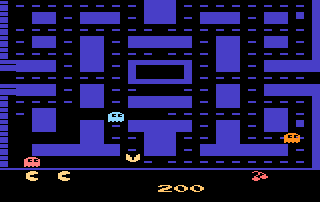
\includegraphics[scale=1.05]{images/pacman.png}
				\caption{Situazione sfavorevole, ma ancora riparabile, guidata per la maggiore dalla voglia di ottenere ricompense istantanee.}
				\label{fig:subpacman}
			\end{subfigure}

			\begin{subfigure}[b]{.49\textwidth}
				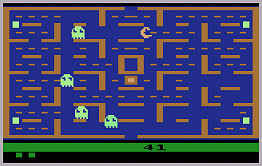
\includegraphics[scale=1.3]{images/pacman1.png}
				\caption{Esempio di scelta sensata, quella di andare a raccogliere punti in un'altra porzione della mappa mentre i fantasmi sono impegnati altrove.}
				\label{fig:subpacman1}
			\end{subfigure}
			
			\label{fig:pacman}
		\end{figure}
	
		\paragraph*{Controesempio} Per quanto riguarda il titolo \textit{Breakout}, in \cite{bib:dqn} viene riportato un caso in cui l'algoritmo individua la furbizia di creare un unico foro nel muro per mandarci la palla dietro (Figura \ref{fig:breakout}).		
		\begin{figure*}[h]
			\centering
			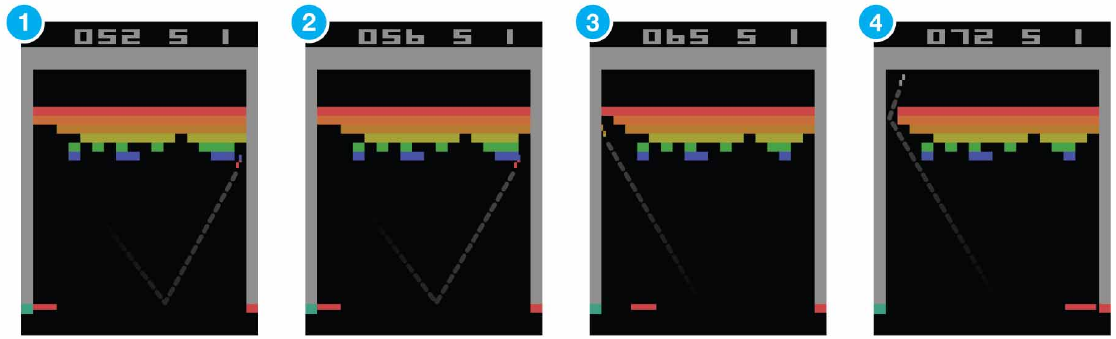
\includegraphics[scale=.65]{images/breakout.png}
			\caption{Dopo un considerevole numero di ore di apprendimento l'algoritmo DQN è in grado di individuare situazioni in cui una sola azione porta numerose ricompense.}
			\label{fig:breakout}
		\end{figure*} 
		In un primo momento potrebbe sembrare che questo sia in contrasto con le conclusioni fatte per quato riguarda \textit{Ms. Pac-Man}. Tuttavia, pensiamo che in \textit{Breakout} la valutazione dell'ottimalità della sequenza di azioni non cambi molto a causa di eventi imprevisti. È questione di ambiente: in \textit{Breakout} non ci sono insidie improvvise (o di qualsiasi altro tipo). A parte questo, il gioco di \textit{Breakout} (così come \textit{Pong}) premiano le \textit{skill} di reattività che vengono perfettamente ricompensate in maniera istantanea. \textit{Pac-Man} (così come \textit{Alien}) non è solo questo.
	
	\subsection{Giochi difficili}
		Un'altro motivo che ci è parso plausibile per la mancanza di prestazioni ottime in alcuni giochi, è perché non sono "semplici" quanto \textit{Breakout} e simili sparatutto (\textit{Space Invader, Deamon Attack}), dove bisogna andare a destra e a sinistra nel momento giusto; si intendono anche i giochi come \textit{Robotank} che sembrano diversi e addirittura in 3D, dove in realtà si tratta sempre di mirare verso destra o sinistra e sparare al momento giusto.
		
		Per dirla in altre parole, ci sono giochi come \textit{Centipede} che aggiungono un grado di difficoltà in più: i nemici sono numerosi e con comportamenti diversi, non si muovono solo in orizzontale ma anche in verticale circondando il giocatore da tutte le direzioni possibili. Come già detto, ci sono tipi di nemici con comportamenti diversi la cui uccisione comporta a un punteggio diverso: sarebbe saggio uccidere il più in fretta possibile le parti del centipede che altrimenti verrebbero a minacciare il giocatore ai lati o dietro le spalle. Tuttavia, ricordiamo che l'algoritmo DQN mappa tutte le ricompense positive al valore $1$. Nelle situazioni più calde alle quali l'algoritmo viene sottoposto (visibile nella Figura \ref{fig:centipede}), esso fa fatica a muoversi in tutte le quattro direzioni continuando a sparare.
		\begin{figure}[t]
			\centering
			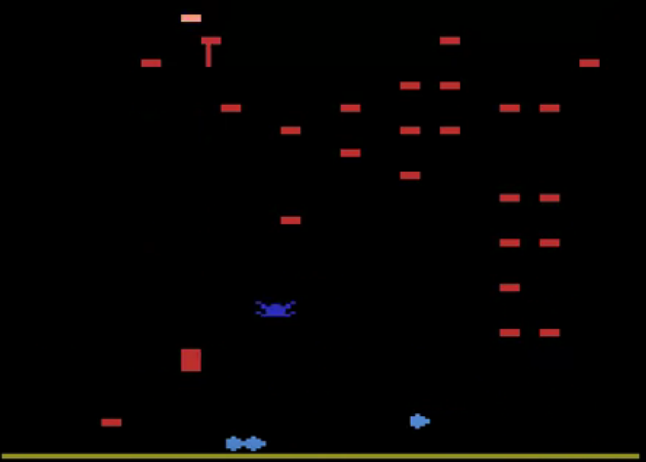
\includegraphics[scale=.5]{images/centipede1.png}
			\caption{Situazione (neanche delle più difficili) in cui l'elfo si ritrova con pezzi di centipede e altri nemici che si muovono a grande velocità intorno al protagonista.}
			\label{fig:centipede}
		\end{figure}
		In più è stato notato che appena dopo la morte del giocatore (punizione $-1$) il gioco si ferma e assegna una ricompensa $+1$ per ogni fungo (quadratini sullo schermo). Questo potrebbe, come minimo, insegnare all'algoritmo che tutto sommato morire non è poi talmente tragico. Esistono in rete discussioni di appassionati del settore che dopo settimane di allenamento non riuscivano a ottenere un agente DQN in \textit{Centipede} che cercasse di muoversi efficientemente sull'asse verticale per evitare il contatto con i nemici.
		\begin{figure*}[ht!]
			\centering
			\caption{Il metodo \texttt{perceive(args)} della classe NeuralQLearner, approssimante la funzione Q con l'ausilio di reti \texttt{CNN}.}
			\lstinputlisting[language={[5.0]Lua}]{code/neuralqlearner.lua}
			\label{code:nql}
		\end{figure*}

\section{Evoluzione degli Algoritmi RL}\label{sec:evoalg}
	%Prioritized Sampling
	
	%On one hand, a more efficient sampling method should emphasize the transitions from which the agent can learn the most. And we all know that transi-tions with positive rewards are more informative and valuable for learning. So we assign these transitions with higher priority to be sampled during training. This	modification of sampling can make transitions with positive rewards be sampled more frequently so as to learn optimal policies faster. On the other hand, we 		add an explicit penalty term to every transition being accessed to reduce the probability of being sampled again. The degrees of punishment will be higher with the increase of sampled times in order to make parts of the transitions never been sampled recently have chances to be reused in time. More importantly, we set the priority of sampling by measuring the magnitude of rewards higher than the latter. + average score + better learning rate
	
	% aggiornamento continuo articolo https://arxiv.org/pdf/1509.02971.pdf
	
	--- DQN
	double
	prioritized sampling
	epsilon	
	
	dove non si usa q-learning (o experience replay) ma policy gradient
	
	--- A3C

	Spiegare l'evoluzione dell'argomento. (non è tutto qui, preferiremmo completare il quadro con.....)
	===
	Unlike policy gradient methods, which attempt to learn functions which directly map an observation to an action, Q-Learning attempts to learn the value of being in a given state, and taking a specific action there.

	\section{Conclusioni}
	
\begin{thebibliography}{99}	
	\bibitem{bib:dqn}
		Volodymyr Mnih, Koray Kavukcuoglu and David Silver,
		\newblock \emph{Human-level control through deep reinforcement learning},
		2015.
		
	\bibitem{bib:chollet2015keras}
		Chollet, Fran\c{c}ois,
		\newblock \emph{Keras},
		\url{https://github.com/fchollet/keras},
		2015

\end{thebibliography}

\end{document}
